\documentclass[12pt, a4paper]{article}

% ── Packages ──────────────────────────────────────────────────────
\usepackage[utf8]{inputenc}
\usepackage[T1]{fontenc}
\usepackage{amsmath, amssymb, amsthm}
\usepackage{mathtools}
\usepackage{enumitem}
\usepackage{tikz}
\usetikzlibrary{calc, positioning, arrows.meta, fit, patterns, decorations.pathreplacing}
\usepackage{geometry}
\geometry{margin=2.4cm}
\usepackage{xcolor}
\usepackage{tcolorbox}
\tcbuselibrary{theorems, skins, breakable}
\usepackage{booktabs}
\usepackage{hyperref}
\hypersetup{colorlinks=true, linkcolor=blue!60!black, urlcolor=blue!60!black}

\setlength{\parindent}{0pt}
\setlength{\parskip}{6pt}

% ── Colours ───────────────────────────────────────────────────────
\definecolor{setA}{RGB}{66, 133, 244}   % blue
\definecolor{setB}{RGB}{234, 67, 53}    % red
\definecolor{setC}{RGB}{251, 188, 4}    % yellow
\definecolor{theoryBg}{RGB}{232, 245, 253}
\definecolor{theoryFrame}{RGB}{66, 133, 244}
\definecolor{stmtBg}{RGB}{255, 243, 224}
\definecolor{stmtFrame}{RGB}{230, 126, 34}
\definecolor{ansBg}{RGB}{232, 250, 232}
\definecolor{ansFrame}{RGB}{39, 174, 96}

% ── Environments ──────────────────────────────────────────────────
\newtcolorbox{theorybox}[1][]{%
  colback=theoryBg, colframe=theoryFrame,
  fonttitle=\bfseries, title={\small Theory Recap: #1},
  breakable, enhanced, arc=2mm,
  left=5pt, right=5pt, top=5pt, bottom=5pt
}

\newtcolorbox{problembox}{%
  colback=stmtBg, colframe=stmtFrame,
  fonttitle=\bfseries, title={\small Problem Statement},
  breakable, enhanced, arc=2mm,
  left=5pt, right=5pt, top=5pt, bottom=5pt
}

\newtcolorbox{answerbox}{%
  colback=ansBg, colframe=ansFrame,
  arc=2mm, left=5pt, right=5pt, top=3pt, bottom=3pt
}

\newcommand{\Z}{\mathbb{Z}}
\newcommand{\R}{\mathbb{R}}
\newcommand{\N}{\mathbb{N}}
\newcommand{\Q}{\mathbb{Q}}
\newcommand{\powset}[1]{2^{#1}}
\newcommand{\comp}[1]{\overline{#1}}
\newcommand{\symdiff}{\mathbin{\triangle}}

% ── Title ─────────────────────────────────────────────────────────
\title{\textbf{Practice 4 --- Functions (Mappings)}\\[4pt]
       \large Solutions to Selected Problems\\[2pt]
       \normalsize Problems 2, 4, 5, 6, 10, 12, 19, 22, 24, 25}
\author{Discrete Mathematics --- QYSU}
\date{}

\begin{document}
\maketitle
\tableofcontents
\newpage

% ══════════════════════════════════════════════════════════════════
\section{Problem 2 --- Domain and Range of Real Functions}
% ══════════════════════════════════════════════════════════════════

\begin{theorybox}[Domain and Range]
For a function $f : \R \to \R$ given by a formula $f(x) = \ldots$\,:
\begin{itemize}[nosep]
  \item The \textbf{domain} $\operatorname{Dom}(f)$ is the set of all $x \in \R$
        for which the formula is defined (no division by zero, no square root
        of a negative number, etc.).
  \item The \textbf{range} (image) $\operatorname{Ran}(f) = \{f(x) \mid x \in \operatorname{Dom}(f)\}$
        is the set of all values actually attained by $f$.
\end{itemize}

\medskip
\textbf{Common restrictions:}
\begin{center}
\renewcommand{\arraystretch}{1.3}
\begin{tabular}{lll}
\toprule
\textbf{Expression} & \textbf{Restriction} & \textbf{Reason} \\
\midrule
$\sqrt{g(x)}$ & $g(x) \ge 0$ & square root of negative undefined in $\R$ \\
$1/g(x)$ & $g(x) \neq 0$ & division by zero undefined \\
$1/\sqrt{g(x)}$ & $g(x) > 0$ & both restrictions combined \\
\bottomrule
\end{tabular}
\end{center}
\end{theorybox}

\begin{problembox}
Let $f : \R \to \R$. Find the domain and range of:
\begin{enumerate}[label=(\alph*), nosep]
  \item $f(x) = x^2 + 3$
  \item $f(x) = \sqrt{x+2}$
  \item $f(x) = \dfrac{1}{\sqrt{x-2}}$
  \item $f(x) = |x|$
  \item $f(x) = \dfrac{1}{x^2+2}$
  \item $f(x) = \dfrac{1}{x^2-2}$
\end{enumerate}
\end{problembox}

\subsection*{Solution}

\textbf{(a)\; $f(x) = x^2 + 3$.}

No restrictions on $x$: every real number can be squared.
\[
  \operatorname{Dom}(f) = \R.
\]
Since $x^2 \ge 0$ for all $x \in \R$, we have $f(x) = x^2 + 3 \ge 3$.
The minimum value $3$ is attained at $x = 0$.
As $x \to \pm\infty$, $f(x) \to +\infty$, and by continuity every value $\ge 3$ is attained.
\[
  \operatorname{Ran}(f) = [3, +\infty).
\]

\begin{answerbox}
$\operatorname{Dom}(f) = \R, \quad \operatorname{Ran}(f) = [3, +\infty).$
\end{answerbox}

\bigskip
\textbf{(b)\; $f(x) = \sqrt{x+2}$.}

We need $x + 2 \ge 0$, i.e.\ $x \ge -2$.
\[
  \operatorname{Dom}(f) = [-2, +\infty).
\]
At $x = -2$: $f(-2) = 0$. As $x \to +\infty$, $f(x) \to +\infty$.
Since $\sqrt{\cdot}$ is continuous and non-negative:
\[
  \operatorname{Ran}(f) = [0, +\infty).
\]

\begin{answerbox}
$\operatorname{Dom}(f) = [-2, +\infty), \quad \operatorname{Ran}(f) = [0, +\infty).$
\end{answerbox}

\bigskip
\textbf{(c)\; $f(x) = \dfrac{1}{\sqrt{x-2}}$.}

We need $x - 2 > 0$ (strict inequality: the square root must be positive since it appears in the denominator), i.e.\ $x > 2$.
\[
  \operatorname{Dom}(f) = (2, +\infty).
\]
As $x \to 2^+$: $\sqrt{x-2} \to 0^+$, so $f(x) \to +\infty$.
As $x \to +\infty$: $\sqrt{x-2} \to +\infty$, so $f(x) \to 0^+$.
Since $f$ is continuous and strictly decreasing on $(2, +\infty)$, it takes every positive value:
\[
  \operatorname{Ran}(f) = (0, +\infty).
\]

\begin{answerbox}
$\operatorname{Dom}(f) = (2, +\infty), \quad \operatorname{Ran}(f) = (0, +\infty).$
\end{answerbox}

\bigskip
\textbf{(d)\; $f(x) = |x|$.}

The absolute value is defined for all real numbers.
\[
  \operatorname{Dom}(f) = \R.
\]
Since $|x| \ge 0$ for all $x$, and $|0| = 0$, and $|x| \to +\infty$ as $x \to \pm\infty$:
\[
  \operatorname{Ran}(f) = [0, +\infty).
\]

\begin{answerbox}
$\operatorname{Dom}(f) = \R, \quad \operatorname{Ran}(f) = [0, +\infty).$
\end{answerbox}

\bigskip
\textbf{(e)\; $f(x) = \dfrac{1}{x^2+2}$.}

Since $x^2 + 2 \ge 2 > 0$ for all $x \in \R$, there is no division by zero.
\[
  \operatorname{Dom}(f) = \R.
\]
Since $x^2 + 2 \ge 2$, we have $f(x) = \frac{1}{x^2+2} \le \frac{1}{2}$.
The maximum $\frac{1}{2}$ is attained at $x = 0$.
As $x \to \pm\infty$, $f(x) \to 0^+$, but $f(x) > 0$ for all $x$.
By continuity, every value in $(0, \frac{1}{2}]$ is attained.
\[
  \operatorname{Ran}(f) = \left(0,\; \tfrac{1}{2}\right].
\]

\begin{answerbox}
$\operatorname{Dom}(f) = \R, \quad \operatorname{Ran}(f) = \bigl(0,\, \frac{1}{2}\bigr].$
\end{answerbox}

\bigskip
\textbf{(f)\; $f(x) = \dfrac{1}{x^2-2}$.}

We need $x^2 - 2 \neq 0$, i.e.\ $x \neq \pm\sqrt{2}$.
\[
  \operatorname{Dom}(f) = \R \setminus \{-\sqrt{2},\; \sqrt{2}\}.
\]
To find the range, set $y = \frac{1}{x^2 - 2}$ and solve for $x^2$:
\[
  y(x^2 - 2) = 1 \implies x^2 = \frac{1}{y} + 2 = \frac{1 + 2y}{y}.
\]
We need $y \neq 0$ and $x^2 = \frac{1+2y}{y} \ge 0$.

Analyzing the sign of $\frac{1+2y}{y}$:
\begin{itemize}[nosep]
  \item $y > 0$: need $1 + 2y > 0$, which holds for all $y > 0$. So $y \in (0, +\infty)$.
  \item $y < 0$: need $1 + 2y < 0$ (numerator and denominator both negative), i.e.\ $y < -\frac{1}{2}$. So $y \in (-\infty, -\frac{1}{2})$.
\end{itemize}
At $x = 0$: $f(0) = \frac{1}{-2} = -\frac{1}{2}$, so $y = -\frac{1}{2}$ is attained.
\[
  \operatorname{Ran}(f) = \left(-\infty,\; -\tfrac{1}{2}\right] \cup (0, +\infty).
\]

\begin{answerbox}
$\operatorname{Dom}(f) = \R \setminus \{-\sqrt{2},\, \sqrt{2}\}, \quad
 \operatorname{Ran}(f) = \bigl(-\infty,\, -\tfrac{1}{2}\bigr] \cup (0, +\infty).$
\end{answerbox}

% ══════════════════════════════════════════════════════════════════
\newpage
\section{Problem 4 --- Composition of Functions}
% ══════════════════════════════════════════════════════════════════

\begin{theorybox}[Function Composition]
Given $f, g : \R \to \R$, the \textbf{composition} $f \circ g$ is defined by:
\[
  (f \circ g)(x) = f\bigl(g(x)\bigr).
\]
\textbf{Read right to left:} first apply $g$, then apply $f$ to the result.

\begin{center}
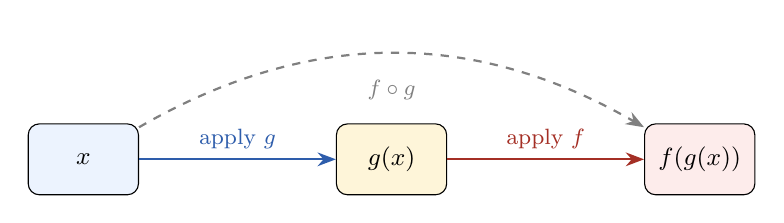
\begin{tikzpicture}[>=Stealth, font=\small, node distance=2.5cm]
  \node[draw, rounded corners, fill=setA!10, minimum width=1.4cm, minimum height=0.9cm] (X) {$x$};
  \node[draw, rounded corners, fill=setC!15, minimum width=1.4cm, minimum height=0.9cm, right=of X] (GX) {$g(x)$};
  \node[draw, rounded corners, fill=setB!10, minimum width=1.4cm, minimum height=0.9cm, right=of GX] (FGX) {$f(g(x))$};
  \draw[->, thick, setA!70!black] (X) -- (GX)
    node[midway, above, font=\footnotesize]{apply $g$};
  \draw[->, thick, setB!70!black] (GX) -- (FGX)
    node[midway, above, font=\footnotesize]{apply $f$};
  \draw[->, thick, gray, dashed, bend left=30] (X) to
    node[midway, below=6pt, font=\footnotesize]{$f \circ g$} (FGX);
\end{tikzpicture}
\end{center}

\textbf{Warning:} In general, $f \circ g \neq g \circ f$ --- composition is not commutative!
\end{theorybox}

\begin{problembox}
Let $f, g : \R \to \R$. Find $f \circ g$ and $g \circ f$ if:
\begin{enumerate}[label=(\alph*), nosep]
  \item $f(x) = x^2 + 1$, \quad $g(x) = x + 3$
  \item $f(x) = \sqrt{x^2 + 2}$, \quad $g(x) = x^2 + 3$
  \item $f(x) = \dfrac{1}{x}$, \quad $g(x) = 2x + 3$
\end{enumerate}
\end{problembox}

\subsection*{Solution}

\textbf{(a)\; $f(x) = x^2 + 1$, \;$g(x) = x + 3$.}

\[
  (f \circ g)(x) = f(g(x)) = f(x+3) = (x+3)^2 + 1 = x^2 + 6x + 9 + 1 = x^2 + 6x + 10.
\]
\[
  (g \circ f)(x) = g(f(x)) = g(x^2+1) = (x^2+1) + 3 = x^2 + 4.
\]

\begin{answerbox}
$(f \circ g)(x) = x^2 + 6x + 10, \qquad (g \circ f)(x) = x^2 + 4.$
\end{answerbox}

\bigskip
\textbf{(b)\; $f(x) = \sqrt{x^2 + 2}$, \;$g(x) = x^2 + 3$.}

\[
  (f \circ g)(x) = f(g(x)) = f(x^2 + 3) = \sqrt{(x^2+3)^2 + 2} = \sqrt{x^4 + 6x^2 + 9 + 2} = \sqrt{x^4 + 6x^2 + 11}.
\]
\[
  (g \circ f)(x) = g(f(x)) = g\!\left(\sqrt{x^2+2}\right) = \left(\sqrt{x^2+2}\right)^2 + 3 = x^2 + 2 + 3 = x^2 + 5.
\]

\begin{answerbox}
$(f \circ g)(x) = \sqrt{x^4 + 6x^2 + 11}, \qquad (g \circ f)(x) = x^2 + 5.$
\end{answerbox}

\bigskip
\textbf{(c)\; $f(x) = \dfrac{1}{x}$, \;$g(x) = 2x + 3$.}

\[
  (f \circ g)(x) = f(g(x)) = f(2x+3) = \frac{1}{2x+3}, \qquad x \neq -\tfrac{3}{2}.
\]
\[
  (g \circ f)(x) = g(f(x)) = g\!\left(\frac{1}{x}\right) = \frac{2}{x} + 3 = \frac{2 + 3x}{x}, \qquad x \neq 0.
\]

\begin{answerbox}
$(f \circ g)(x) = \dfrac{1}{2x+3}\;(x \neq -\frac{3}{2}), \qquad
 (g \circ f)(x) = \dfrac{2+3x}{x}\;(x \neq 0).$
\end{answerbox}

% ══════════════════════════════════════════════════════════════════
\newpage
\section{Problem 5 --- Inverse Functions}
% ══════════════════════════════════════════════════════════════════

\begin{theorybox}[Inverse Function]
If $f : A \to B$ is a bijection, then $f$ has an \textbf{inverse function} $f^{-1} : B \to A$ satisfying:
\[
  f^{-1}(y) = x \iff f(x) = y.
\]
\textbf{Algorithm to find $f^{-1}$:}
\begin{enumerate}[nosep]
  \item Write $y = f(x)$.
  \item Solve for $x$ in terms of $y$.
  \item Swap the names: the expression for $x$ in terms of $y$ is $f^{-1}(y)$.
\end{enumerate}

\textbf{Verification:} $f^{-1}(f(x)) = x$ and $f(f^{-1}(y)) = y$.
\end{theorybox}

\begin{problembox}
Find the inverse relation for:
\begin{enumerate}[label=(\alph*), nosep]
  \item $f(x) = \dfrac{x+4}{2}$
  \item $f(x) = x^3$
  \item $f(x) = \dfrac{x-2}{x+3}$
\end{enumerate}
\end{problembox}

\subsection*{Solution}

\textbf{(a)\; $f(x) = \dfrac{x+4}{2}$.}

Set $y = \frac{x+4}{2}$. Solve for $x$:
\[
  2y = x + 4 \implies x = 2y - 4.
\]
\[
  \boxed{f^{-1}(y) = 2y - 4.}
\]

\emph{Verification:}\; $f(f^{-1}(y)) = f(2y-4) = \frac{(2y-4)+4}{2} = \frac{2y}{2} = y.\;\checkmark$

$f^{-1}(f(x)) = f^{-1}\!\left(\frac{x+4}{2}\right) = 2 \cdot \frac{x+4}{2} - 4 = x + 4 - 4 = x.\;\checkmark$

\begin{answerbox}
$f^{-1}(x) = 2x - 4.$
\end{answerbox}

\bigskip
\textbf{(b)\; $f(x) = x^3$.}

Set $y = x^3$. Solve for $x$:
\[
  x = \sqrt[3]{y} = y^{1/3}.
\]
\[
  \boxed{f^{-1}(y) = \sqrt[3]{y}.}
\]

\emph{Verification:}\; $f(f^{-1}(y)) = (\sqrt[3]{y})^3 = y.\;\checkmark$ \quad
$f^{-1}(f(x)) = \sqrt[3]{x^3} = x.\;\checkmark$

\begin{answerbox}
$f^{-1}(x) = \sqrt[3]{x}.$
\end{answerbox}

\bigskip
\textbf{(c)\; $f(x) = \dfrac{x-2}{x+3}$, \quad $x \neq -3$.}

Set $y = \frac{x-2}{x+3}$. Solve for $x$:
\begin{align*}
  y(x+3) &= x - 2 \\
  yx + 3y &= x - 2 \\
  yx - x &= -2 - 3y \\
  x(y - 1) &= -(2 + 3y) \\
  x &= \frac{-(2+3y)}{y-1} = \frac{2+3y}{1-y}, \qquad y \neq 1.
\end{align*}
Note that $f(x) = 1$ has no solution (it would require $x - 2 = x + 3$, i.e.\ $-2 = 3$), confirming $1 \notin \operatorname{Ran}(f)$.
\[
  \boxed{f^{-1}(y) = \frac{2 + 3y}{1 - y}, \qquad y \neq 1.}
\]

\emph{Verification:}\;
$f(f^{-1}(y)) = f\!\left(\frac{2+3y}{1-y}\right)
= \frac{\frac{2+3y}{1-y} - 2}{\frac{2+3y}{1-y} + 3}
= \frac{2+3y - 2(1-y)}{2+3y + 3(1-y)}
= \frac{2+3y-2+2y}{2+3y+3-3y}
= \frac{5y}{5} = y.\;\checkmark$

\begin{answerbox}
$f^{-1}(x) = \dfrac{2+3x}{1-x}, \quad x \neq 1.$
\end{answerbox}

% ══════════════════════════════════════════════════════════════════
\newpage
\section{Problem 6 --- Injectivity, Surjectivity, Bijectivity}
% ══════════════════════════════════════════════════════════════════

\begin{theorybox}[Injective, Surjective, Bijective]
Let $f : A \to B$.
\begin{itemize}[nosep]
  \item \textbf{Injective} (one-to-one): $f(x_1) = f(x_2) \implies x_1 = x_2$.
        Equivalently, $x_1 \neq x_2 \implies f(x_1) \neq f(x_2)$.
        \emph{Horizontal line test:} every horizontal line meets the graph at most once.
  \item \textbf{Surjective} (onto): $\forall\, y \in B,\; \exists\, x \in A : f(x) = y$.
        Equivalently, $\operatorname{Ran}(f) = B$.
  \item \textbf{Bijective}: both injective and surjective.
\end{itemize}

\begin{center}
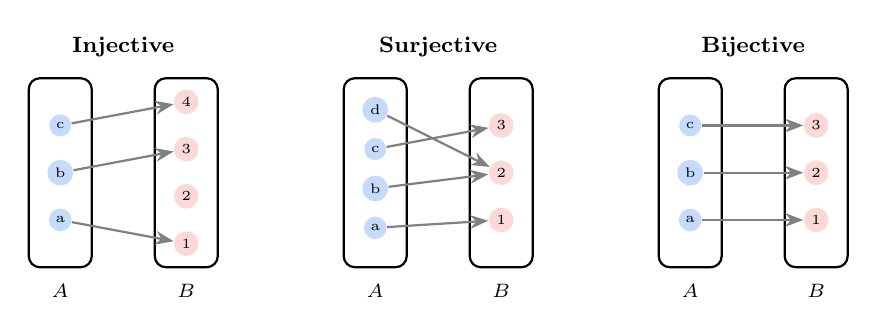
\begin{tikzpicture}[>=Stealth, font=\small]
  % Injective
  \begin{scope}[xshift=0cm]
    \node[font=\footnotesize\bfseries] at (1.2, 2.5) {Injective};
    \draw[thick, rounded corners] (0, -0.3) rectangle (0.8, 2.1);
    \draw[thick, rounded corners] (1.6, -0.3) rectangle (2.4, 2.1);
    \node[font=\scriptsize] at (0.4, -0.6) {$A$};
    \node[font=\scriptsize] at (2.0, -0.6) {$B$};
    \foreach \y/\lbl in {0.3/a, 0.9/b, 1.5/c}
      \node[fill=setA!30, circle, inner sep=1.5pt, font=\tiny] (L\lbl) at (0.4, \y) {\lbl};
    \foreach \y/\lbl in {0.0/1, 0.6/2, 1.2/3, 1.8/4}
      \node[fill=setB!20, circle, inner sep=1.5pt, font=\tiny] (R\lbl) at (2.0, \y) {\lbl};
    \draw[->, thick, gray] (La) -- (R1);
    \draw[->, thick, gray] (Lb) -- (R3);
    \draw[->, thick, gray] (Lc) -- (R4);
  \end{scope}
  % Surjective
  \begin{scope}[xshift=4cm]
    \node[font=\footnotesize\bfseries] at (1.2, 2.5) {Surjective};
    \draw[thick, rounded corners] (0, -0.3) rectangle (0.8, 2.1);
    \draw[thick, rounded corners] (1.6, -0.3) rectangle (2.4, 2.1);
    \node[font=\scriptsize] at (0.4, -0.6) {$A$};
    \node[font=\scriptsize] at (2.0, -0.6) {$B$};
    \foreach \y/\lbl in {0.2/a, 0.7/b, 1.2/c, 1.7/d}
      \node[fill=setA!30, circle, inner sep=1.5pt, font=\tiny] (L\lbl) at (0.4, \y) {\lbl};
    \foreach \y/\lbl in {0.3/1, 0.9/2, 1.5/3}
      \node[fill=setB!20, circle, inner sep=1.5pt, font=\tiny] (R\lbl) at (2.0, \y) {\lbl};
    \draw[->, thick, gray] (La) -- (R1);
    \draw[->, thick, gray] (Lb) -- (R2);
    \draw[->, thick, gray] (Lc) -- (R3);
    \draw[->, thick, gray] (Ld) -- (R2);
  \end{scope}
  % Bijective
  \begin{scope}[xshift=8cm]
    \node[font=\footnotesize\bfseries] at (1.2, 2.5) {Bijective};
    \draw[thick, rounded corners] (0, -0.3) rectangle (0.8, 2.1);
    \draw[thick, rounded corners] (1.6, -0.3) rectangle (2.4, 2.1);
    \node[font=\scriptsize] at (0.4, -0.6) {$A$};
    \node[font=\scriptsize] at (2.0, -0.6) {$B$};
    \foreach \y/\lbl in {0.3/a, 0.9/b, 1.5/c}
      \node[fill=setA!30, circle, inner sep=1.5pt, font=\tiny] (L\lbl) at (0.4, \y) {\lbl};
    \foreach \y/\lbl in {0.3/1, 0.9/2, 1.5/3}
      \node[fill=setB!20, circle, inner sep=1.5pt, font=\tiny] (R\lbl) at (2.0, \y) {\lbl};
    \draw[->, thick, gray] (La) -- (R1);
    \draw[->, thick, gray] (Lb) -- (R2);
    \draw[->, thick, gray] (Lc) -- (R3);
  \end{scope}
\end{tikzpicture}
\end{center}
\end{theorybox}

\begin{problembox}
Determine which of the following mappings $f : \R \to \R$ are injective,
surjective, or bijective:
\begin{enumerate}[label=(\alph*), nosep]
  \item $f(x) = |x|$
  \item $f(x) = x^2 + 4$
  \item $f(x) = x^3 + 6$
  \item $f(x) = x + |x|$
  \item $f(x) = x(x-2)(x+2)$
\end{enumerate}
\end{problembox}

\subsection*{Solution}

\textbf{(a)\; $f(x) = |x|$.}

\emph{Not injective:}\; $f(1) = |1| = 1 = |-1| = f(-1)$, but $1 \neq -1$.

\emph{Not surjective:}\; $|x| \ge 0$ for all $x$, so no $x$ satisfies $f(x) = -1$.
The range is $[0, +\infty) \neq \R$.

\begin{answerbox}
$f(x) = |x|$: neither injective nor surjective (hence not bijective).
\end{answerbox}

\bigskip
\textbf{(b)\; $f(x) = x^2 + 4$.}

\emph{Not injective:}\; $f(1) = 5 = f(-1)$, but $1 \neq -1$.

\emph{Not surjective:}\; $x^2 + 4 \ge 4$ for all $x$, so no $x$ satisfies $f(x) = 0$.
The range is $[4, +\infty) \neq \R$.

\begin{answerbox}
$f(x) = x^2 + 4$: neither injective nor surjective (hence not bijective).
\end{answerbox}

\bigskip
\textbf{(c)\; $f(x) = x^3 + 6$.}

\emph{Injective:}\; Suppose $f(x_1) = f(x_2)$. Then $x_1^3 + 6 = x_2^3 + 6$,
so $x_1^3 = x_2^3$. Since the cube function is strictly increasing on $\R$,
this implies $x_1 = x_2$.

\emph{Surjective:}\; Given any $y \in \R$, we need $x^3 + 6 = y$, i.e.\
$x = \sqrt[3]{y - 6}$. Since the cube root is defined for all real numbers,
such $x$ always exists.

\begin{answerbox}
$f(x) = x^3 + 6$: \textbf{bijective} (both injective and surjective).
\end{answerbox}

\bigskip
\textbf{(d)\; $f(x) = x + |x|$.}

First, let us simplify:
\[
  f(x) = x + |x| = \begin{cases} 2x & \text{if } x \ge 0, \\ 0 & \text{if } x < 0. \end{cases}
\]

\emph{Not injective:}\; $f(-1) = 0 = f(-2)$, but $-1 \neq -2$.
(In fact, $f(x) = 0$ for all $x < 0$.)

\emph{Not surjective:}\; For $x \ge 0$, $f(x) = 2x \ge 0$.
For $x < 0$, $f(x) = 0$. So $f(x) \ge 0$ for all $x$,
and no $x$ satisfies $f(x) = -1$. The range is $[0, +\infty) \neq \R$.

\begin{answerbox}
$f(x) = x + |x|$: neither injective nor surjective (hence not bijective).
\end{answerbox}

\bigskip
\textbf{(e)\; $f(x) = x(x-2)(x+2) = x^3 - 4x$.}

\emph{Not injective:}\; $f(0) = 0$ and $f(2) = 2 \cdot 0 \cdot 4 = 0$,
so $f(0) = f(2) = 0$ but $0 \neq 2$.

\emph{Surjective:}\; $f(x) = x^3 - 4x$ is a cubic polynomial with positive leading coefficient.
As $x \to -\infty$, $f(x) \to -\infty$, and as $x \to +\infty$, $f(x) \to +\infty$.
By the Intermediate Value Theorem, every $y \in \R$ is attained.

\begin{answerbox}
$f(x) = x(x-2)(x+2)$: surjective but \textbf{not injective} (hence not bijective).
\end{answerbox}

% ══════════════════════════════════════════════════════════════════
\newpage
\section{Problem 10 --- Kernel of a Mapping is an Equivalence Relation}
% ══════════════════════════════════════════════════════════════════

\begin{theorybox}[Kernel of a Mapping]
Let $f : A \to B$ be a mapping. The \textbf{kernel} of $f$ is the relation on $A$ defined by:
\[
  \operatorname{Ker}(f) = \{(a_1, a_2) \in A \times A \mid f(a_1) = f(a_2)\}.
\]
We write $a_1 \sim a_2$ to mean $(a_1, a_2) \in \operatorname{Ker}(f)$, i.e.\ $f(a_1) = f(a_2)$.

\medskip
An \textbf{equivalence relation} on $A$ is a relation $\sim$ that is:
\begin{enumerate}[nosep]
  \item \textbf{Reflexive:} $a \sim a$ for all $a \in A$.
  \item \textbf{Symmetric:} $a \sim b \implies b \sim a$.
  \item \textbf{Transitive:} $a \sim b \land b \sim c \implies a \sim c$.
\end{enumerate}

\begin{center}
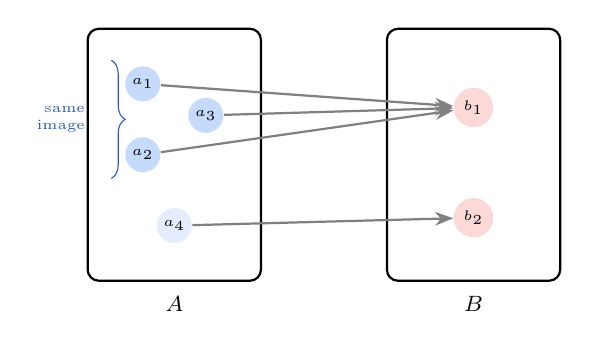
\begin{tikzpicture}[>=Stealth, font=\small]
  \draw[thick, rounded corners] (0, 0) rectangle (2.2, 3.2);
  \draw[thick, rounded corners] (3.8, 0) rectangle (6.0, 3.2);
  \node[font=\footnotesize\bfseries] at (1.1, -0.3) {$A$};
  \node[font=\footnotesize\bfseries] at (4.9, -0.3) {$B$};

  \node[fill=setA!30, circle, inner sep=1.5pt, font=\tiny] (a1) at (0.7, 2.5) {$a_1$};
  \node[fill=setA!30, circle, inner sep=1.5pt, font=\tiny] (a2) at (0.7, 1.6) {$a_2$};
  \node[fill=setA!30, circle, inner sep=1.5pt, font=\tiny] (a3) at (1.5, 2.1) {$a_3$};
  \node[fill=setA!15, circle, inner sep=1.5pt, font=\tiny] (a4) at (1.1, 0.7) {$a_4$};

  \node[fill=setB!20, circle, inner sep=2pt, font=\tiny] (b1) at (4.9, 2.2) {$b_1$};
  \node[fill=setB!20, circle, inner sep=2pt, font=\tiny] (b2) at (4.9, 0.8) {$b_2$};

  \draw[->, thick, gray] (a1) -- (b1);
  \draw[->, thick, gray] (a2) -- (b1);
  \draw[->, thick, gray] (a3) -- (b1);
  \draw[->, thick, gray] (a4) -- (b2);

  % equivalence class brace
  \draw[decorate, decoration={brace, amplitude=5pt, mirror}, setA!70!black]
    (0.3, 1.3) -- (0.3, 2.8)
    node[midway, left=6pt, font=\tiny, align=right]{same\\image};
\end{tikzpicture}
\end{center}
The equivalence classes of $\operatorname{Ker}(f)$ are exactly the \textbf{fibers}
$f^{-1}(\{b\}) = \{a \in A \mid f(a) = b\}$ for $b \in \operatorname{Ran}(f)$.
\end{theorybox}

\begin{problembox}
Prove that for any mapping $f : A \to B$, its kernel $\operatorname{Ker}(f)$ is an equivalence relation on $A$.
\end{problembox}

\subsection*{Solution}

We must verify the three properties of an equivalence relation.
Recall: $a_1 \sim a_2 \iff f(a_1) = f(a_2)$.

\textbf{1. Reflexivity.}\;
Let $a \in A$. Then $f(a) = f(a)$ (equality is reflexive), so $a \sim a$. \checkmark

\textbf{2. Symmetry.}\;
Suppose $a_1 \sim a_2$, i.e.\ $f(a_1) = f(a_2)$.
Then $f(a_2) = f(a_1)$ (equality is symmetric), so $a_2 \sim a_1$. \checkmark

\textbf{3. Transitivity.}\;
Suppose $a_1 \sim a_2$ and $a_2 \sim a_3$, i.e.\ $f(a_1) = f(a_2)$ and $f(a_2) = f(a_3)$.
Then $f(a_1) = f(a_3)$ (equality is transitive), so $a_1 \sim a_3$. \checkmark

\medskip
Since $\operatorname{Ker}(f)$ is reflexive, symmetric, and transitive, it is an equivalence relation on $A$. \qed

\begin{answerbox}
The kernel $\operatorname{Ker}(f)$ inherits reflexivity, symmetry, and transitivity
from the equality relation ``$=$'' on $B$, so it is an equivalence relation on $A$.
\end{answerbox}

% ══════════════════════════════════════════════════════════════════
\newpage
\section{Problem 12 --- $f(x) = \frac{x}{2x+1}$ on $\Q^+$: Injective but Not Surjective}
% ══════════════════════════════════════════════════════════════════

\begin{theorybox}[Injectivity and Surjectivity --- Proof Techniques]
\textbf{To prove injectivity:}\;
Assume $f(x_1) = f(x_2)$ and show $x_1 = x_2$ (direct proof),
or assume $x_1 \neq x_2$ and show $f(x_1) \neq f(x_2)$ (contrapositive).

\textbf{To disprove surjectivity:}\;
Find a specific $y$ in the codomain for which $f(x) = y$ has no solution in the domain.

\textbf{To prove surjectivity:}\;
Given arbitrary $y$ in the codomain, solve $f(x) = y$ and verify $x$ lies in the domain.
\end{theorybox}

\begin{problembox}
Let $f : \Q^+ \to \Q^+$ be defined by $f(x) = \dfrac{x}{2x+1}$.
Prove that $f$ is injective but not surjective.
\end{problembox}

\subsection*{Solution}

\textbf{Injectivity.}\;
Let $x_1, x_2 \in \Q^+$ and suppose $f(x_1) = f(x_2)$:
\[
  \frac{x_1}{2x_1 + 1} = \frac{x_2}{2x_2 + 1}.
\]
Cross-multiplying (the denominators are positive since $x_1, x_2 > 0$):
\[
  x_1(2x_2 + 1) = x_2(2x_1 + 1).
\]
Expanding:
\[
  2x_1 x_2 + x_1 = 2x_1 x_2 + x_2.
\]
Subtracting $2x_1 x_2$ from both sides:
\[
  x_1 = x_2.
\]
Therefore $f$ is injective. \qed

\bigskip
\textbf{Not surjective.}\;
We claim that $y = \frac{1}{2}$ is in $\Q^+$ but not in $\operatorname{Ran}(f)$.

Suppose for contradiction that there exists $x \in \Q^+$ with $f(x) = \frac{1}{2}$:
\[
  \frac{x}{2x+1} = \frac{1}{2} \implies 2x = 2x + 1 \implies 0 = 1.
\]
This is a contradiction. Therefore no $x \in \Q^+$ satisfies $f(x) = \frac{1}{2}$.

\medskip
More generally, for any $x > 0$:
\[
  f(x) = \frac{x}{2x+1} = \frac{1}{2 + \frac{1}{x}} < \frac{1}{2},
\]
since $\frac{1}{x} > 0$, so $2 + \frac{1}{x} > 2$, and thus $\frac{1}{2+\frac{1}{x}} < \frac{1}{2}$.
Therefore $\operatorname{Ran}(f) \subseteq \bigl(0, \frac{1}{2}\bigr)$, so $f$ is not surjective onto $\Q^+$. \qed

\begin{answerbox}
$f(x) = \frac{x}{2x+1}$ on $\Q^+$ is \textbf{injective} (by cross-multiplication)
but \textbf{not surjective} (e.g., $y = \frac{1}{2}$ is not in the range, since $f(x) < \frac{1}{2}$ for all $x > 0$).
\end{answerbox}

% ══════════════════════════════════════════════════════════════════
\newpage
\section{Problem 19 --- $f(A \cap B) = f(A) \cap f(B)$ Iff $f$ Is Injective}
% ══════════════════════════════════════════════════════════════════

\begin{theorybox}[Images of Intersections]
For any mapping $f : X \to Y$ and subsets $A, B \subseteq X$:
\[
  f(A \cap B) \subseteq f(A) \cap f(B) \qquad\text{always holds.}
\]
However, equality $f(A \cap B) = f(A) \cap f(B)$ does \textbf{not} hold in general.
It holds for \emph{all} $A, B \subseteq X$ if and only if $f$ is \textbf{injective}.

\begin{center}
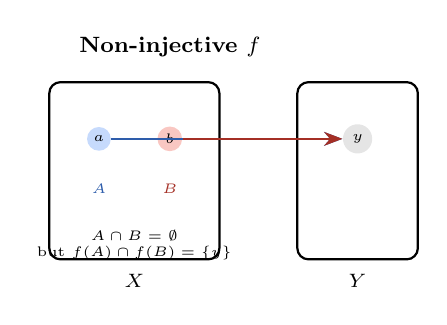
\begin{tikzpicture}[>=Stealth, font=\small, scale=0.9]
  % Non-injective case
  \begin{scope}[xshift=0cm]
    \node[font=\footnotesize\bfseries] at (1.5, 2.8) {Non-injective $f$};
    \draw[thick, rounded corners] (-0.2, -0.2) rectangle (2.2, 2.3);
    \draw[thick, rounded corners] (3.3, -0.2) rectangle (5.0, 2.3);
    \node[font=\scriptsize] at (1.0, -0.5) {$X$};
    \node[font=\scriptsize] at (4.15, -0.5) {$Y$};

    \node[fill=setA!30, circle, inner sep=1.5pt, font=\tiny] (a) at (0.5, 1.5) {$a$};
    \node[fill=setB!30, circle, inner sep=1.5pt, font=\tiny] (b) at (1.5, 1.5) {$b$};
    \node[font=\tiny, setA!70!black] at (0.5, 0.8) {$A$};
    \node[font=\tiny, setB!70!black] at (1.5, 0.8) {$B$};

    \node[fill=gray!20, circle, inner sep=2pt, font=\tiny] (y) at (4.15, 1.5) {$y$};

    \draw[->, thick, setA!70!black] (a) -- (y);
    \draw[->, thick, setB!70!black] (b) -- (y);

    \node[font=\tiny, align=center] at (1.0, 0.0) {$A \cap B = \emptyset$\\but $f(A)\cap f(B) = \{y\}$};
  \end{scope}
\end{tikzpicture}
\end{center}
\end{theorybox}

\begin{problembox}
For which mappings does $f(A \cap B) = f(A) \cap f(B)$ hold for all subsets $A, B$ of the domain?

Answer: injective mappings. Prove both directions.
\end{problembox}

\subsection*{Solution}

\textbf{Direction 1: If $f$ is injective, then $f(A \cap B) = f(A) \cap f(B)$.}

The inclusion $f(A \cap B) \subseteq f(A) \cap f(B)$ holds for any function (if $x \in A \cap B$, then $f(x) \in f(A)$ and $f(x) \in f(B)$).

We prove the reverse inclusion $f(A) \cap f(B) \subseteq f(A \cap B)$.

Let $y \in f(A) \cap f(B)$. Then:
\begin{itemize}[nosep]
  \item $y \in f(A)$: there exists $a \in A$ with $f(a) = y$.
  \item $y \in f(B)$: there exists $b \in B$ with $f(b) = y$.
\end{itemize}
Since $f(a) = y = f(b)$ and $f$ is injective, we conclude $a = b$.
Call this common element $c = a = b$. Then $c \in A$ and $c \in B$, so $c \in A \cap B$.
Therefore $y = f(c) \in f(A \cap B)$.

This shows $f(A) \cap f(B) \subseteq f(A \cap B)$, completing the proof of equality. \qed

\bigskip
\textbf{Direction 2: If $f(A \cap B) = f(A) \cap f(B)$ for all $A, B$, then $f$ is injective.}

We prove the contrapositive: if $f$ is not injective, then there exist $A, B$ with $f(A \cap B) \neq f(A) \cap f(B)$.

Suppose $f$ is not injective. Then there exist $x_1 \neq x_2$ in the domain with $f(x_1) = f(x_2)$.
Set $A = \{x_1\}$ and $B = \{x_2\}$. Then:
\begin{itemize}[nosep]
  \item $A \cap B = \emptyset$ (since $x_1 \neq x_2$), so $f(A \cap B) = f(\emptyset) = \emptyset$.
  \item $f(A) = \{f(x_1)\}$ and $f(B) = \{f(x_2)\} = \{f(x_1)\}$,
        so $f(A) \cap f(B) = \{f(x_1)\} \neq \emptyset$.
\end{itemize}
Therefore $f(A \cap B) \neq f(A) \cap f(B)$. \qed

\begin{answerbox}
$f(A \cap B) = f(A) \cap f(B)$ holds for all $A, B$ if and only if $f$ is injective.
\end{answerbox}

% ══════════════════════════════════════════════════════════════════
\newpage
\section{Problem 22 --- Disjoint Subsets with Equal Images}
% ══════════════════════════════════════════════════════════════════

\begin{theorybox}[Images of Disjoint Sets]
If $f : A \to B$ is \textbf{not} injective, then different elements can map to the same
image. This means disjoint subsets of the domain can have overlapping --- or even equal --- images.
\end{theorybox}

\begin{problembox}
Is it possible for $f : A \to B$ and disjoint non-empty $X_1, X_2 \subseteq A$
(i.e.\ $X_1 \cap X_2 = \emptyset$, $X_1 \neq \emptyset$, $X_2 \neq \emptyset$)
to have $f(X_1) = f(X_2)$?
\end{problembox}

\subsection*{Solution}

\textbf{Yes}, this is possible. We give a concrete example.

Let $A = \{1, 2, 3, 4\}$, $B = \{a, b\}$, and define $f$ by:
\[
  f(1) = a, \quad f(2) = b, \quad f(3) = a, \quad f(4) = b.
\]
Take $X_1 = \{1, 2\}$ and $X_2 = \{3, 4\}$.

\begin{center}
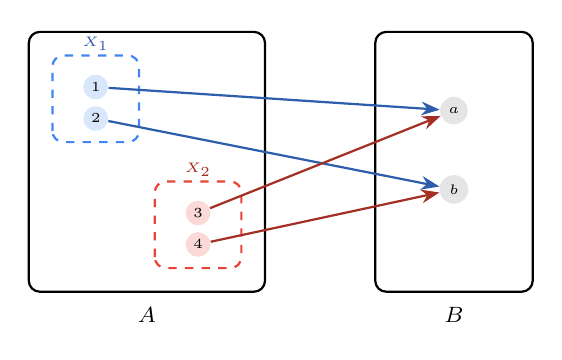
\begin{tikzpicture}[>=Stealth, font=\small]
  \draw[thick, rounded corners] (-0.2, -0.3) rectangle (2.8, 3.0);
  \draw[thick, rounded corners] (4.2, -0.3) rectangle (6.2, 3.0);
  \node[font=\footnotesize\bfseries] at (1.3, -0.6) {$A$};
  \node[font=\footnotesize\bfseries] at (5.2, -0.6) {$B$};

  % X1 box
  \draw[thick, setA, dashed, rounded corners] (0.1, 1.6) rectangle (1.2, 2.7);
  \node[font=\tiny, setA!70!black] at (0.65, 2.85) {$X_1$};
  \node[fill=setA!20, circle, inner sep=1.5pt, font=\tiny] (n1) at (0.65, 2.3) {$1$};
  \node[fill=setA!20, circle, inner sep=1.5pt, font=\tiny] (n2) at (0.65, 1.9) {$2$};

  % X2 box
  \draw[thick, setB, dashed, rounded corners] (1.4, 0.0) rectangle (2.5, 1.1);
  \node[font=\tiny, setB!70!black] at (1.95, 1.25) {$X_2$};
  \node[fill=setB!20, circle, inner sep=1.5pt, font=\tiny] (n3) at (1.95, 0.7) {$3$};
  \node[fill=setB!20, circle, inner sep=1.5pt, font=\tiny] (n4) at (1.95, 0.3) {$4$};

  % B elements
  \node[fill=gray!20, circle, inner sep=2pt, font=\tiny] (a) at (5.2, 2.0) {$a$};
  \node[fill=gray!20, circle, inner sep=2pt, font=\tiny] (b) at (5.2, 1.0) {$b$};

  \draw[->, thick, setA!70!black] (n1) -- (a);
  \draw[->, thick, setA!70!black] (n2) -- (b);
  \draw[->, thick, setB!70!black] (n3) -- (a);
  \draw[->, thick, setB!70!black] (n4) -- (b);
\end{tikzpicture}
\end{center}

Then:
\begin{itemize}[nosep]
  \item $X_1 \cap X_2 = \{1,2\} \cap \{3,4\} = \emptyset$. \checkmark
  \item $f(X_1) = \{f(1), f(2)\} = \{a, b\}$.
  \item $f(X_2) = \{f(3), f(4)\} = \{a, b\}$.
  \item $f(X_1) = f(X_2) = \{a, b\}$. \checkmark
\end{itemize}

\begin{answerbox}
\textbf{Yes.} Disjoint non-empty subsets can have equal images when $f$ is not injective.
Example: $f(1)=a,\; f(2)=b,\; f(3)=a,\; f(4)=b$ with $X_1=\{1,2\}$, $X_2=\{3,4\}$.
\end{answerbox}

% ══════════════════════════════════════════════════════════════════
\newpage
\section{Problem 24 --- Preimages of Disjoint Sets}
% ══════════════════════════════════════════════════════════════════

\begin{theorybox}[Preimages Preserve Set Operations]
For any function $f : A \to B$ and subsets $Y_1, Y_2 \subseteq B$, the \textbf{preimage}
$f^{-1}(Y) = \{x \in A \mid f(x) \in Y\}$ satisfies:
\begin{itemize}[nosep]
  \item $f^{-1}(Y_1 \cup Y_2) = f^{-1}(Y_1) \cup f^{-1}(Y_2)$
  \item $f^{-1}(Y_1 \cap Y_2) = f^{-1}(Y_1) \cap f^{-1}(Y_2)$
  \item $f^{-1}(Y_1 \setminus Y_2) = f^{-1}(Y_1) \setminus f^{-1}(Y_2)$
\end{itemize}
These hold for \emph{any} function --- no injectivity or surjectivity is required!
\end{theorybox}

\begin{problembox}
Is it true that for $f : A \to B$, if $Y_1 \cap Y_2 = \emptyset$, then
$f^{-1}(Y_1) \cap f^{-1}(Y_2) = \emptyset$?
\end{problembox}

\subsection*{Solution}

\textbf{Yes}, this is always true.

\begin{proof}
Suppose $Y_1 \cap Y_2 = \emptyset$. We use the identity $f^{-1}(Y_1 \cap Y_2) = f^{-1}(Y_1) \cap f^{-1}(Y_2)$.

Since $Y_1 \cap Y_2 = \emptyset$:
\[
  f^{-1}(Y_1) \cap f^{-1}(Y_2) = f^{-1}(Y_1 \cap Y_2) = f^{-1}(\emptyset) = \emptyset.
\]

Alternatively, we can prove it directly. Suppose for contradiction that there exists
$x \in f^{-1}(Y_1) \cap f^{-1}(Y_2)$. Then:
\begin{itemize}[nosep]
  \item $x \in f^{-1}(Y_1) \implies f(x) \in Y_1$.
  \item $x \in f^{-1}(Y_2) \implies f(x) \in Y_2$.
\end{itemize}
So $f(x) \in Y_1 \cap Y_2 = \emptyset$, which is a contradiction since no element belongs to the empty set.
\end{proof}

\begin{answerbox}
\textbf{Yes.} If $Y_1 \cap Y_2 = \emptyset$, then $f^{-1}(Y_1) \cap f^{-1}(Y_2) = \emptyset$.
This follows from the fact that preimages preserve intersections.
\end{answerbox}

% ══════════════════════════════════════════════════════════════════
\newpage
\section{Problem 25 --- $f(f^{-1}(Y)) \subseteq Y$}
% ══════════════════════════════════════════════════════════════════

\begin{theorybox}[Image of a Preimage]
For $f : A \to B$ and $Y \subseteq B$:
\[
  f(f^{-1}(Y)) \subseteq Y \qquad\text{always holds.}
\]
Equality $f(f^{-1}(Y)) = Y$ holds for all $Y \subseteq B$ if and only if $f$ is \textbf{surjective}.

\medskip
\textbf{Intuition:}\; $f^{-1}(Y)$ captures all elements in $A$ that map into $Y$.
Applying $f$ again maps them back into $Y$ --- but some elements of $Y$ may have
\emph{no preimage}, so they are ``lost.''

\begin{center}
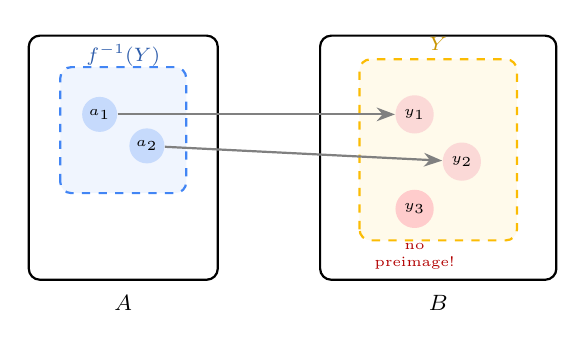
\begin{tikzpicture}[>=Stealth, font=\small]
  \draw[thick, rounded corners] (-0.2, -0.3) rectangle (2.2, 2.8);
  \draw[thick, rounded corners] (3.5, -0.3) rectangle (6.5, 2.8);
  \node[font=\footnotesize\bfseries] at (1.0, -0.6) {$A$};
  \node[font=\footnotesize\bfseries] at (5.0, -0.6) {$B$};

  % Y subset in B
  \draw[thick, setC, dashed, rounded corners, fill=setC!8] (4.0, 0.2) rectangle (6.0, 2.5);
  \node[font=\scriptsize, setC!80!black] at (5.0, 2.7) {$Y$};

  \node[fill=setB!20, circle, inner sep=2pt, font=\tiny] (y1) at (4.7, 1.8) {$y_1$};
  \node[fill=setB!20, circle, inner sep=2pt, font=\tiny] (y2) at (5.3, 1.2) {$y_2$};
  \node[fill=red!20, circle, inner sep=2pt, font=\tiny] (y3) at (4.7, 0.6) {$y_3$};

  % preimage in A
  \draw[thick, setA, dashed, rounded corners, fill=setA!8] (0.2, 0.8) rectangle (1.8, 2.4);
  \node[font=\scriptsize, setA!70!black] at (1.0, 2.55) {$f^{-1}(Y)$};

  \node[fill=setA!30, circle, inner sep=1.5pt, font=\tiny] (a1) at (0.7, 1.8) {$a_1$};
  \node[fill=setA!30, circle, inner sep=1.5pt, font=\tiny] (a2) at (1.3, 1.4) {$a_2$};

  \draw[->, thick, gray] (a1) -- (y1);
  \draw[->, thick, gray] (a2) -- (y2);

  \node[font=\tiny, red!70!black, align=center] at (4.7, 0.0) {no\\preimage!};
\end{tikzpicture}
\end{center}
Here $f(f^{-1}(Y)) = \{y_1, y_2\} \subsetneq \{y_1, y_2, y_3\} = Y$.
\end{theorybox}

\begin{problembox}
Prove that for $f : A \to B$ and $Y \subseteq B$:
\[
  f(f^{-1}(Y)) \subseteq Y.
\]
Give an example where equality does not hold.
\end{problembox}

\subsection*{Solution}

\textbf{Proof of $f(f^{-1}(Y)) \subseteq Y$.}

Let $y \in f(f^{-1}(Y))$. By definition of image, there exists $x \in f^{-1}(Y)$
such that $f(x) = y$. By definition of preimage, $x \in f^{-1}(Y)$ means $f(x) \in Y$.
Therefore $y = f(x) \in Y$. \qed

\bigskip
\textbf{Example where equality fails.}

Let $A = \{1\}$, $B = \{a, b\}$, and define $f : A \to B$ by $f(1) = a$.
Take $Y = \{a, b\} = B$.

Then:
\[
  f^{-1}(Y) = f^{-1}(\{a,b\}) = \{x \in A \mid f(x) \in \{a,b\}\} = \{1\}.
\]
\[
  f(f^{-1}(Y)) = f(\{1\}) = \{f(1)\} = \{a\}.
\]
But $Y = \{a, b\}$. So:
\[
  f(f^{-1}(Y)) = \{a\} \subsetneq \{a, b\} = Y.
\]
The element $b \in Y$ has no preimage under $f$ (since $f$ is not surjective), so it is ``lost.''

\begin{answerbox}
\textbf{Proof:} If $y \in f(f^{-1}(Y))$, then $y = f(x)$ for some $x \in f^{-1}(Y)$,
which means $f(x) \in Y$, i.e.\ $y \in Y$.

\textbf{Counterexample to equality:}\; $A = \{1\}$, $B = \{a,b\}$, $f(1) = a$, $Y = B$.
Then $f(f^{-1}(Y)) = \{a\} \subsetneq \{a,b\} = Y$.

Equality holds for all $Y$ iff $f$ is surjective.
\end{answerbox}

\end{document}
